\documentclass[a4paper,12pt]{article}

\usepackage{mystyle}

\graphicspath{ {images/} }

\usetikzlibrary{arrows.meta}

\definecolor{my-green}{RGB}{0, 153, 0}
\definecolor{my-pink}{RGB}{248, 23, 62}
\definecolor{my-red}{RGB}{176, 0, 0}
\definecolor{my-blue}{RGB}{0, 0, 153}
\definecolor{my-grey}{RGB}{128,128,128}


\author{Алексеев Василий}

\title{Семинар 8}
\date{27 октября 2022}


\begin{document}
  \maketitle
  
  \tableofcontents

  \thispagestyle{empty}
  
  \newpage
  
  \pagenumbering{arabic}


  \section{Касательная к кривой второго порядка}
  
  Для эллипса, заданного в канонической системе координат уравнением
  \[
    \frac{x^2}{a^2} + \frac{y^2}{b^2} = 1
  \]
  уравнение касательной в точке $(x_0, y_0)$ эллипса выглядит так
  \[
    \boxed{\frac{xx_0}{a^2} + \frac{yy_0}{b^2} = 1}
  \]
  
  Для гиперболы, заданной в канонической системе координат уравнением
  \[
    \frac{x^2}{a^2} - \frac{y^2}{b^2} = 1
  \]
  уравнение касательной в точке $(x_0, y_0)$ гиперболы выглядит так
  \[
    \boxed{\frac{xx_0}{a^2} - \frac{yy_0}{b^2} = 1}
  \]
  
  И для параболы, заданной в канонической системе координат уравнением
  \[
    y^2 = 2px
  \]
  уравнение касательной в точке $(x_0, y_0)$ параболы выглядит так
  \[
    \boxed{yy_0 = p (x + x_0)}
  \]
  
  
  \subsection{\# 8.2(3)}
  
  Составить уравнение касательной к кривой
  \[
    xy = k
  \]

  \begin{solution}
    Можно продифференцировать обе части уравнения кривой в некоторой точке $(x_0, y_0)$, принадлежащей кривой:
    \[
      d(xy)\bigm|_{(x_0, y_0)} = d(k)\bigm|_{(x_0, y_0)}
    \]
    Откуда
    \[
      x_0 dy + y_0 dx = 0 \Rightarrow \frac{dy}{dx} = -\frac{y_0}{x_0}
    \]
    То есть тангенс угла наклона касательной к кривой в точке $(x_0, y_0)$ равен $-\dfrac{y_0}{x_0}$.
    С другой стороны, тот же тангенс для касательной можно посчитать просто как отношение приращений $(y \hm- y_0)$ и $(x \hm- x_0)$ для некоторой точки $(x, y)$ касательной:
    \[
      \frac{y - y_0}{x - x_0} = -\frac{y_0}{x_0}
    \]
    
    Проводя упрощения и учитывая, что для исходной точки выполняется $x_0 y_0 \hm= k$, получаем
    \[
      y_0 x + x_0 y = 2k
    \]
  \end{solution}
  
  
  \subsection{\# 8.9(1)}
  
  Какие точки на кривой второго порядка
  \[
    \frac{27}{28} x^2 + \frac{9}{7} y^2 = 1
  \]
  удалены на наименьшее расстояние от прямой
  \[
    l\colon 3x + 4y + 5 = 0
  \]
  Найти это расстояние.
  
  \begin{solution}
    \begin{figure}[h]
      \centering

      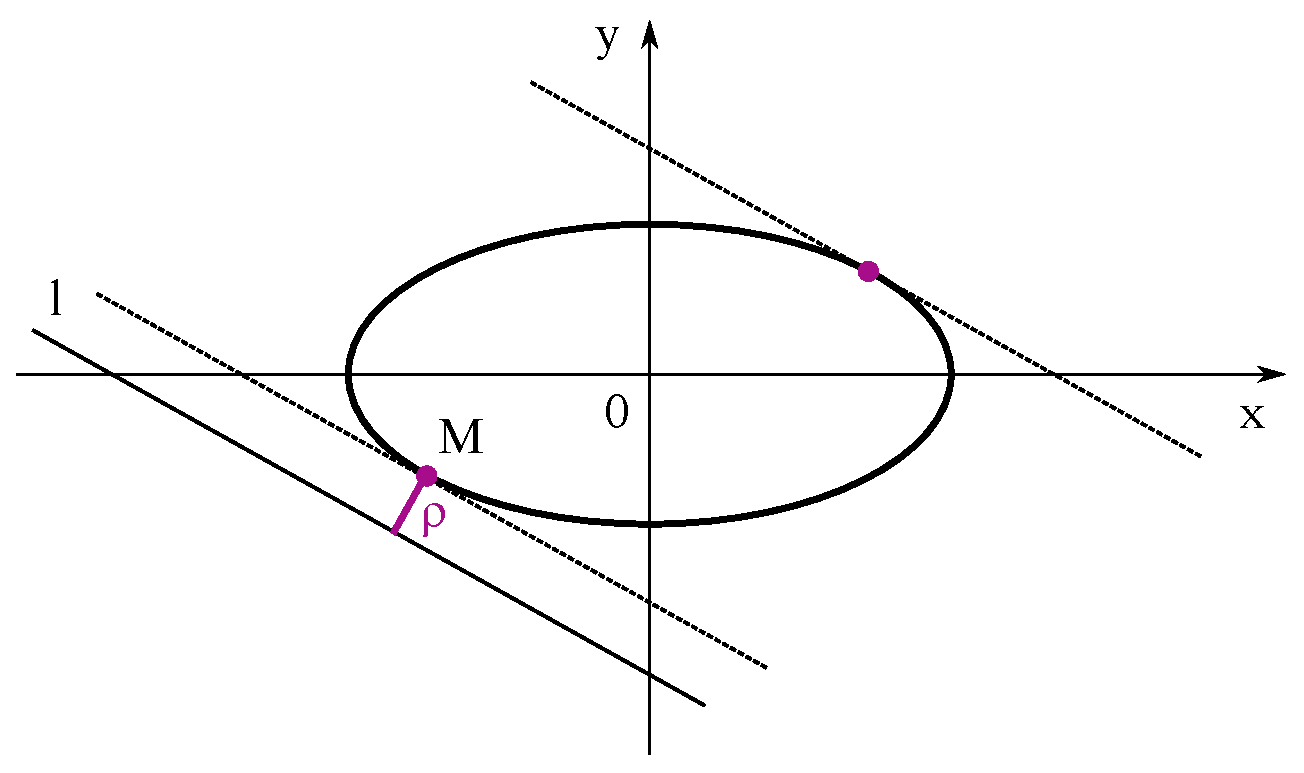
\includegraphics[width=0.8\textwidth]{ellipse-8-9}
    
      \caption{Прямая $l$ не пересекает эллипс.}
      \label{fig:ellipse-8-9}
    \end{figure}
    
    Из рисунка (\ref{fig:ellipse-8-9}) видно, что прямая $l$ и эллипс не пересекаются, поэтому минимальное расстояние не нулевое.
    Также из рисунка понятно, что расстояние от точки $M(x_0, y_0)$ эллипса до прямой $l$ будет минимальным в том случае, когда касательная к эллипсу в точке $M$ параллельна прямой $l$\footnote{``Очевидно''. А вообще, потому что эллипс ``хороший'': выпуклый (отрезок, соединяющий любые две точки эллипса, лежит внутри эллипса) и угол наклона касательной от точки к точке эллипса меняется непрерывно (то есть нет ``пропусков'' углов).}.
    Но таких точек, очевидно, у эллипса две (при этом если расстояние от одной из них до прямой $l$ будет минимальным, то от другой, наоборот, расстояние будет максимальным среди точек эллипса).
    
    Уравнение касательной к эллипсу в точке $M(x_0, y_0)$:
    \[
      \frac{27}{28} x_0 x + \frac{9}{7} y_0 y = 1
    \]
    
    Сравнивая уравнение касательной с уравнением прямой, выводим условие параллельности касательной и прямой:
    \[
      \frac{27/28 x_0}{3} = \frac{9/7 y_0}{4}
    \]
    
    Откуда получаем
    $
      x_0 \hm= y_0
    $.
    При этом $(x_0, y_0)$~---~точка эллипса:
    \[
      \frac{27}{28} x_0^2 + \frac{9}{7} y_0^2 = 1
    \]
    
    В итоге
    \[
      \left\{
        \begin{aligned}
          &x_0 = \pm \frac{2}{3}\\
          &y_0 = \pm \frac{2}{3}
        \end{aligned}
      \right.
    \]
    
    Из рисунка (\ref{fig:ellipse-8-9}) видно, что подходит точка $\left(-\dfrac{2}{3}, -\dfrac{2}{3}\right)$.
    
    Расстояние от найденной точки до прямой $l$ в канонической системе координат эллипса (которая прямоугольная) вычисляется по формуле:
    \[
      \rho{\bigl((x_0, y_0), l\bigr)} = \frac{\left|3 \cdot \left(-\frac{2}{3}\right) + 4 \cdot \left(-\frac{2}{3}\right) + 5\right|}{\sqrt{3^2 + 4^2}} = \ldots = \frac{1}{15}
    \]
  \end{solution}
  
  
  \subsection{\# 8.24(1)}
  
  Составить уравнения касательных к эллипсу, заданному в канонической системе координат уравнением
  \[
    \frac{x^2}{18} + \frac{y^2}{8} = 1
  \]
  проходящих через точку $P(-6, 0)$.
  
  \begin{solution}
    \begin{figure}[h]
      \centering

      \includegraphics[width=0.8\textwidth]{ellipse-8-24}
    
      \caption{Касательные к эллипсу, проходящие через одну точку на оси $X$ в канонической системе координат эллипса.}
      \label{fig:ellipse-8-24}
    \end{figure}
    
    Уравнение касательной к эллипсу в точке $M(x_0, y_0)$, которая проходит через точку $P(-6, 0)$ (\ref{fig:ellipse-8-24}):
    \[
      \frac{-6 x_0}{18} + 0 = 1 \Rightarrow x_0 = -3
    \]
    
    Подставляя найденную координату $x_0$ в уравнение эллипса, находим координаты $y_0$:
    \[
      \frac{(-3)^2}{18} + \frac{y_0^2}{8} = 1 \Rightarrow y_0 = \pm 2
    \]
    
    И уравнения касательных
    \[
      -2x \pm 3y - 12 = 0
    \]
  \end{solution}
  

  \section{Приведение уравнения кривой к каноническому виду}
  
  Общий вид уравнения кривой второго порядка:
  \begin{equation}\label{eq:second-order-curve}
    \left\{
      \begin{aligned}
        &Ax^2 + 2B xy + Cy^2 + 2Dx + 2Ey + F = 0\\
        &A^2 + B^2 + C^2 > 0
      \end{aligned}
    \right.
  \end{equation}
  
  Всего есть девять канонических уравнений кривых второго порядка\footnote{См., например книжку Беклемишева~Д.~В. или Задачник.}:
  
  \begin{enumerate}
    \item\label{enum:ellipse} Эллипс
      \[
        \left\{
          \begin{aligned}
            &\frac{x^2}{a^2} + \frac{y^2}{b^2} = 1\\
            &a \geq b > 0
          \end{aligned}
        \right.
      \]
    \item ``Мнимый эллипс''
      \[
        \frac{x^2}{a^2} + \frac{y^2}{b^2} = -1,\quad a \not= 0,\ b \not= 0
      \]
    \item ``Пара мнимых пересекающихся прямых''
      \[
        \frac{x^2}{a^2} + \frac{y^2}{b^2} = 0,\quad a \not= 0,\ b \not= 0
      \]
    
    % https://tex.stackexchange.com/a/186191/135045
    \noindent\textcolor{my-grey}{\rule{0.8\textwidth}{1pt}}

    \item\label{enum:hyperbola} Гипербола
      \[
        \frac{x^2}{a^2} - \frac{y^2}{b^2} = 1,\quad a > 0,\ b > 0
      \]
    \item Пара пересекающихся прямых
      \[
        \frac{x^2}{a^2} - \frac{y^2}{b^2} = 0,\quad a \not= 0,\ b \not= 0
      \]
    
    \noindent\textcolor{my-grey}{\rule{0.8\textwidth}{1pt}}
    
    \item\label{enum:parabola} Парабола
      \[
        y^2 = 2px, \quad p > 0
      \]
    \item Пара параллельных прямых
      \[
        y^2 = a^2,\quad a \not= 0
      \]
    \item ``Пара мнимых параллельных прямых''
      \[
        y^2 = -a^2,\quad a \not= 0
      \]
    \item Пара совпавших прямых
      \[
        y^2 = 0
      \]
  \end{enumerate}
  
  Чтобы привести кривую к каноническому виду, можно придерживаться следующего алгоритма:
  \begin{enumerate}
    \setcounter{enumi}{-1}
    \item Перейти к прямоугольной системе координат (если она ещё не прямоугольная)\footnote{В задачах изначальная система координат будет считаться прямоугольной, если не сказано противное!}.
    \item \emph{Повернуть} систему координат так, чтобы исчез член с произведением $xy$.
    \item Далее, в зависимости от ситуации, надо \emph{перенести начало} системы координат так, чтобы исчезли либо линейные члены, либо свободный член.
    \item И в конце, опять же в зависимости от ситуации, может потребоваться ещё одно-два небольших действия, например изменение порядка координат (чего можно достичь поворотом на $\dfrac{\pi}{2}$, чтобы не менялась ориентация базиса).
  \end{enumerate}
  
  Центром кривой второго порядка называется точка $(x_0, y_0)$, такая что
  \[
    F(x_0 + \alpha, y_0 + \beta) = F(x_0 - \alpha, y_0 - \beta)
  \]
  где $F(\cdot, \cdot) \hm= 0$~---~уравнение кривой, а $\alpha$ и $\beta$~---~любые числа.
  Можно показать, что центр симметрии кривой~---~это почти то же самое, что и её центр (только центр в некоторых случая может существовать, а центр симметрии~---~нет).
  Если подставить в уравнение (\ref{eq:second-order-curve}) сдвинутые на $\pm \alpha$ и $\pm \beta$ координаты $(x_0, y_0)$ и приравнять, как в определении центра, то получим
  \[
    \alpha (Ax_0 + Bx_0 + D) + \beta (Bx_0 + Cy_0 + E) = 0
  \]
  откуда система уравнений для нахождения координат центра:
  \begin{equation}\label{eq:second-order-curve-center}
    \left\{
      \begin{aligned}
        &Ax_0 + Bx_0 + D = 0\\
        &Bx_0 + Cy_0 + E = 0
      \end{aligned}
    \right.
  \end{equation}
  
  Центр существует и единствен, если определитель системы отличен от нуля:
  \[
    \delta = \begin{vmatrix}A & B \\ B & C\end{vmatrix} \not= 0
  \]
  В этом случае кривая называется \emph{центральной}.
  
  При этом $\delta \hm> 0$ соответствует кривым \emph{эллиптического типа}: от эллипса до гиперболы в списке кривых (\ref{enum:ellipse}),~---~$\delta \hm< 0$ соответствует кривым \emph{гиперболического типа}: от гиперболы до параболы в списке кривых (\ref{enum:hyperbola}),~---~и $\delta \hm= 0$ соответствует кривым \emph{параболического типа}: от параболы и далее (\ref{enum:parabola}).
  
  
  \subsection{\# 9.1(3)}
  
  Определить тип кривой второго порядка.
  Составить её каноническое уравнение и найти каноническую систему координат.
  Изначально кривая задана в некоторой \emph{прямоугольной системе координат} уравнением:
  \begin{equation}\label{eq:problem-9-1}
    9x^2 + 4y^2 + 6x - 4y - 2 = 0
  \end{equation}
  
  \begin{solution}
    В уравнении нет члена с $xy$, поэтому поворот делать не придётся.
    Видно, что для приведения к каноническому виду надо выделять квадраты:
    \[
      (9x^2 + 2 \cdot 3x + 1) - 1 + (4y^2 - 2 \cdot 2y + 1) - 1 - 2 = 0
    \]
    \[
      (3x + 1)^2 + (2y - 1)^2 = 4
    \]
    
    Нужная замена переменных уже ``почти видна''.
    Остаётся только сделать так, чтобы переход к новой системе координат был именно \emph{параллельным переносом} (без сжатия или растяжения, чтобы система координат оставалась прямоугольной):
    \[
      9 \left(x + \frac{1}{3}\right)^2 + 4 \left(y - \frac{1}{2}\right)^2 = 4
    \]
    
    Проводим теперь уже очевидную замену:
    \[
      \left\{
        \begin{aligned}
          &x' = x + \frac{1}{3}\\
          &y' = y - \frac{1}{2}
        \end{aligned}
      \right.
    \]
    
    И выписываем уравнение кривой в новых координатах:
    \[
      9 x'^2 + 4 y'^2 = 4 \Leftrightarrow \frac{x'^2}{(2/3)^2} + \frac{y'^2}{1^2} = 1
    \]
    
    Это уравнение эллипса, но... снова не каноническое, потому что $2/3 \hm< 1$.
    Забудем про замену $x', y'$.
    Замену координат стоило делать так (дополнительно ещё меняем оси местами\footnote{Стоит только иметь в виду, что при такой ``перемене мест осей'' меняется и ориентация базиса. Чтобы ориентация сохранилась, надо бы было выполнить \emph{поворот} на $\pi/2$. Но решили в этой задаче обойтись без поворота, поэтому опустим)}):
    \[
      \left\{
        \begin{aligned}
          &x' = y - \frac{1}{2}\\
          &y' = x + \frac{1}{3}
        \end{aligned}
      \right.
    \]
    
    И каноническое уравнение эллипса:
    \[
      \frac{x'^2}{1^2} + \frac{y'^2}{(2/3)^2} = 1
    \]
    
    Определим положение начала новой системы координат $O'$ в старой и выражения новых базисных векторов $\bds e_1'$, $\bds e_2'$ через старые $\bds e_1$, $\bds e_2$.
    Для этого надо вывести формулы для обратной замены:
    \[
      \left\{
        \begin{aligned}
          &x = \hphantom{x' + {}} y' - \frac{1}{3}\\
          &y = x' + \hphantom{y' + {}} \frac{1}{2}
        \end{aligned}
      \right.
    \]
    
    Координаты $O'$:
    \[
      \left\{
        \begin{aligned}
          &x = 0 - \frac{1}{3} = -\frac{1}{3}\\
          &y = 0 + \frac{1}{2} = \frac{1}{2}
        \end{aligned}
      \right.
    \]
    
    Компоненты новых базисных в старом базисе:
    \[
      \bds e_1' = (0, 1),\quad \bds e_2' = (1, 0)
    \]
    
    (Поменяли оси, поэтому базисные тоже ``поменялись''.)
  \end{solution}


  \subsection{\# 9.4(1)}
  
  Определить тип кривой второго порядка.
  Составить её каноническое уравнение и найти каноническую систему координат.
  Изначально кривая задана в некоторой \emph{прямоугольной системе координат} уравнением:
  \begin{equation}\label{eq:problem-9-4}
    F(x, y) = 2x^2 - 4xy + 5y^2 + 8x - 2y + 9 = 0
  \end{equation}
  
  \begin{solution}
    \vphantom{}
  
    \emph{Способ I (``канонический'')}.
    
    Тип кривой можно определить либо сразу, либо в самом конце, когда получим каноническое уравнение.
    Давайте отложим на конец (а в другом варианте решения сделаем это сразу).
    
    Первый шаг~---~надо повернуть систему координат так, чтобы исчез член со смешанным произведением переменных $xy$.
    Поворот системы координат:
    \[
      \left\{
        \begin{aligned}
          &x = x' \cos \phi - y' \sin \phi\\
          &y = x' \sin \phi + y' \cos \phi
        \end{aligned}
      \right.
    \]
    
    Подставляем в исходное уравнение и смотрим, что получается как коэффициент при $x'y'$:
    \begin{equation*}
    \begin{split}
      F'(x', y') &= 2 (x' \cos \phi - y' \sin \phi)^2 - 4 (x' \cos \phi - y' \sin \phi) (x' \sin \phi + y' \cos \phi)\\
      &+ 5 (x' \sin \phi + y' \cos \phi)^2 + \ldots
      = (6 \sin\phi \cos\phi - 4 \cos^2 \phi + 4\sin^2 \phi)x' y' + \ldots = 0
    \end{split}
    \end{equation*}
    Откуда получаем условие на угол поворота $\phi$, чтобы коэффициент при $x'y'$ обратился в ноль:
    \[
       3 \sin 2\phi - 4 \cos 2\phi = 0 \Rightarrow \tg 2\phi = \frac{4}{3}
    \]
    
    \begin{figure}[h]
      \centering

      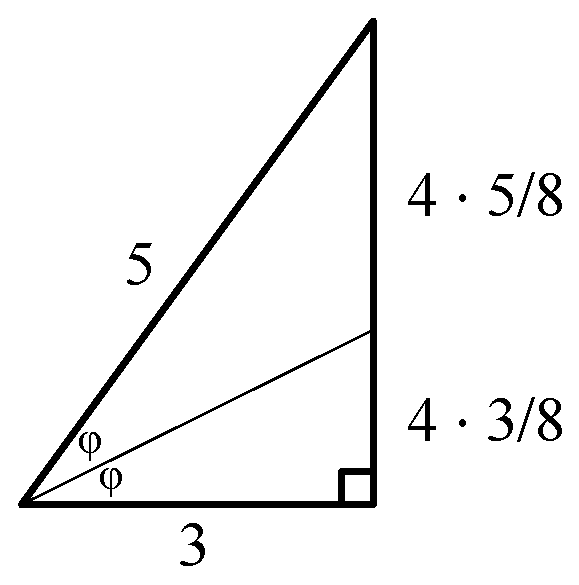
\includegraphics[width=0.25\textwidth]{triangle-9-4}
    
      \caption{К нахождению $\sin\phi$ и $\cos\phi$ по $\tg{2\phi}$, \emph{если считать $2\phi$ острым}.}
      \label{fig:triangle-9-4}
    \end{figure}
    
    Из рисунка (\ref{fig:triangle-9-4}), например, можно найти синус и косинус для одинарного угла (\emph{при условии, что $2\phi$ острый}\footnote{Но можно бы было выбрать и тупой $2\phi$...}):
    \[
      \left\{
        \begin{aligned}
          &\sin\phi = \frac{1}{\sqrt{5}}\\
          &\cos\phi = \frac{2}{\sqrt{5}}
        \end{aligned}
      \right.
    \]
    
    Тогда первая замена:
    \[
      \boxed{
        \left\{
          \begin{aligned}
            &x = \frac{2}{\sqrt{5}} x' - \frac{1}{\sqrt{5}} y'\\
            &y = \frac{1}{\sqrt{5}} x' + \frac{2}{\sqrt{5}} y'
          \end{aligned}
        \right.
      }
    \]
    
    Снова подставляем это представление $x$ и $y$ через $x'$ и $y'$ в исходное уравнение, но на этот раз выписываем все члены, кроме $x'y'$ (так как он должен занулиться):
    \[
      F'(x', y') = \ldots = x'^2 + 6y'^2 + \frac{14x'}{\sqrt{5}} - \frac{12y'}{\sqrt{5}} + 9 = 0
    \]
    
    Далее можно выделить полные квадраты, чтобы избавиться от линейных членов
    \[
      \left(x'^2 + 2 \cdot \frac{7}{\sqrt{5}} x' + \frac{49}{5}\right) - \frac{49}{5}
        + \left(\left(\sqrt{6} y'\right)^2 - 2 \cdot \sqrt{6} y \cdot \frac{6}{\sqrt{30}} + \frac{36}{30}\right) - \frac{36}{30} + 9 = 0
    \]
    \[
      \left(x' + \frac{7}{\sqrt{5}}\right)^2 + \left(\sqrt{6} y' - \frac{6}{\sqrt{30}}\right)^2  = 2
    \]
    \[
      \left(x' + \frac{7}{\sqrt{5}}\right)^2 + 6\left(y' - \frac{1}{\sqrt{5}}\right)^2  = 2
    \]
    
    Откуда видна следующая замена:
    \[
      \boxed{
        \left\{
          \begin{aligned}
            &x'' = x' + \frac{7}{\sqrt{5}}\\
            &y'' = y' - \frac{1}{\sqrt{5}}
          \end{aligned}
        \right.
      }
    \]
    
    Уравнение при этом в переменных $x''$, $y''$ примет вид:
    \[
      x''^2 + 6y''^2 = 2
    \]
    
    Или, уже каноническое:
    \[
      \frac{x''^2}{2} + \frac{y''^2}{1/3} = 1
    \]
    
    Видно, что крива второго порядка~---~эллипс.
    Осталось задать каноническую систему координат, связав её с исходной.
    Можно вывести замену $x$ и $y$ сразу на $x''$ и $y''$~---~тогда станет известна матрица перехода от исходного базиса к новому и положение новой (канонической) системы координат относительно исходной.
    
    Выражая и подставляя из одной замены в другую, получаем
    \[
      \left\{
        \begin{aligned}
          &x = \ldots = \frac{2}{\sqrt{5}}x'' - \frac{1}{\sqrt{5}}y'' - 3\\
          &y = \ldots = \frac{1}{\sqrt{5}}x'' + \frac{2}{\sqrt{5}}y'' - 1
        \end{aligned}
      \right.
    \]
    
    Откуда видны компоненты новых базисных векторов в старом базисе и положение нового начала:
    \[
      \left\{
        \begin{aligned}
          &O'(-3, -1)\\
          &\bds e_1' = \left(\frac{2}{\sqrt{5}}, \frac{1}{\sqrt{5}}\right)\\
          &\bds e_2' = \left(-\frac{1}{\sqrt{5}}, \frac{2}{\sqrt{5}}\right)
        \end{aligned}
      \right.
    \]
    
    
    \emph{Способ II (``через центр'')}.
    
    Если у кривой есть центр, то удобнее начинать замены с переноса начала координат в этот центр.
    Из системы уравнений (\ref{eq:second-order-curve-center}) можно понять, есть у кривой центр или нет.
    И, если есть, найти его координаты
    \[
      \left\{
        \begin{aligned}
          &2x_0 - 2y_0 + 4 = 0\\
          &-2x_0 + 5y_0 - 1 = 0
        \end{aligned}
      \right.
    \]
    
    Определитель системы
    \[
      \delta = \begin{vmatrix}2 & -2 \\ -2 & 5\end{vmatrix} = 6 > 0
    \]
    (из того, что определитель больше нуля, сразу можно заключить, что кривая эллиптического типа).
    Решая далее, например, по методу Крамера, находим
    \[
      \left\{
        \begin{aligned}
          &x_0 = -3\\
          &y_0 = -1
        \end{aligned}
      \right.
    \]
    
    И первая замена~---~перенос начала координат в центр:
    \[
      \left\{
        \begin{aligned}
          &x = -3 + x'\\
          &y = -1 + y'
        \end{aligned}
      \right.
    \]
    
    Подставляя в уравнение (\ref{eq:problem-9-4}), получаем
    \[
      2x'^2 + 5y'^2 - 4x'y' = 2
    \]
    то есть линейные члены ушли.
    Осталось повернуть систему координат.
    Поворот должен быть таким же, как в первом способе решения.
    В итоге
    \[
      x''^2 + 6y''^2 = 2
    \]
    
    Получили то же самое, что и в первый раз, но вычислений пришлось проводить в разы меньше (и вероятность совершить какую-нибудь ошибку тоже была меньше).
    Координаты нового центра при этом стали известны уже на стадии первой замены переменных.
  \end{solution}
  
  
  \section{Дополнение: Ещё задача про касательные}
  
  \subsection{\# 8.29(3)}
  
  Доказать, что пучок света, испущенный из фокуса параболы, отразившись от её стенок, пойдёт параллельно оси параболы.
  
  \begin{solution}
    \begin{figure}[h]
      \centering

      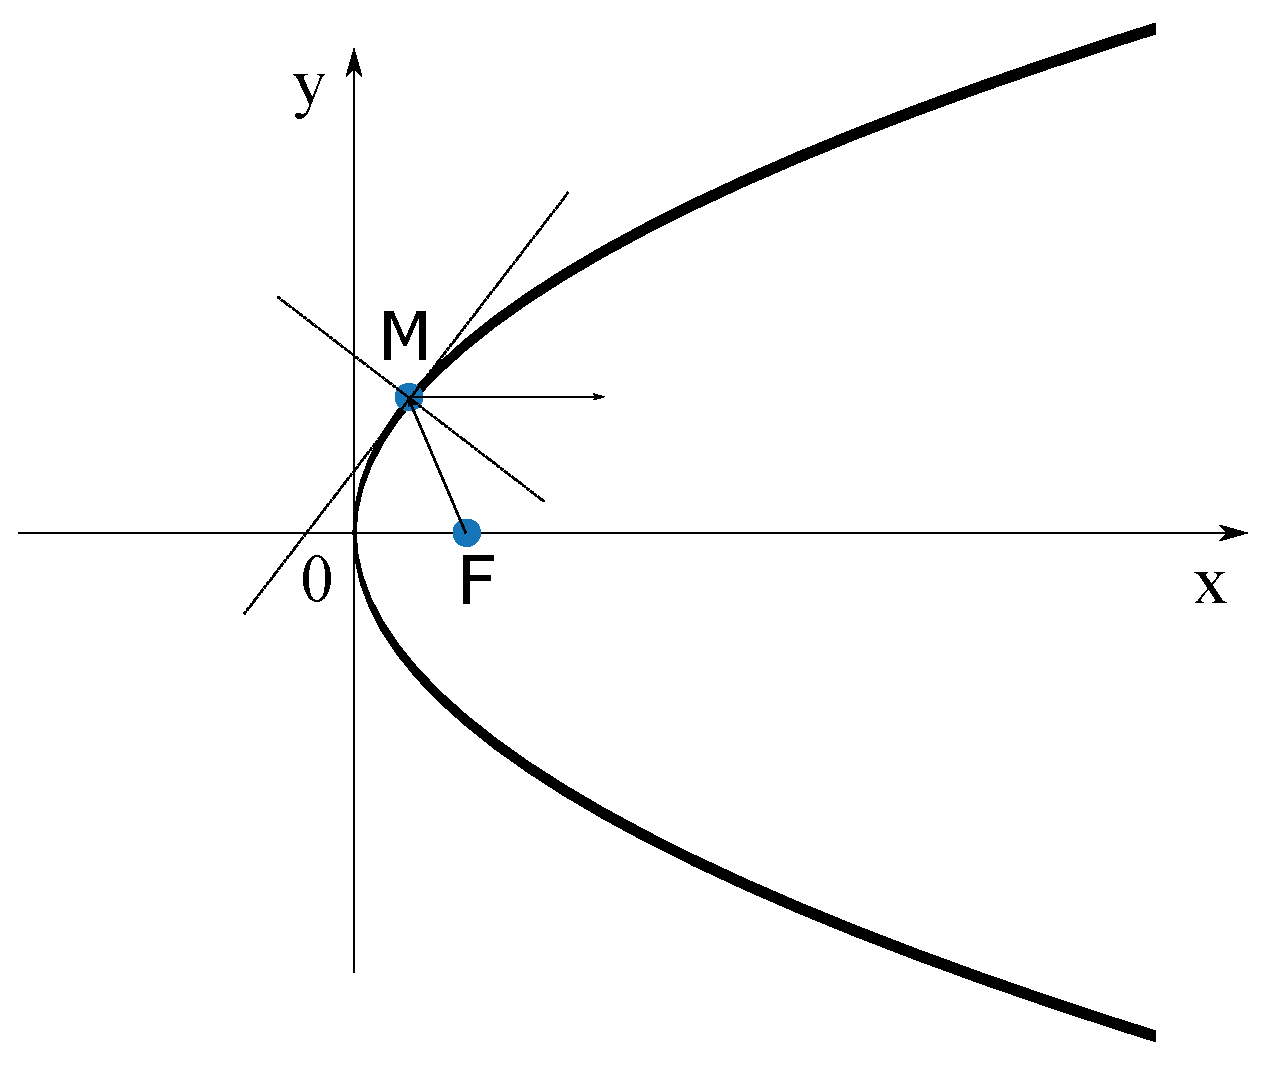
\includegraphics[width=0.5\textwidth]{parabola-8-29}
    
      \caption{Луч, исходящий из фокуса параболы и отражённый далее от её ``стенки''.}
      \label{fig:parabola-8-29}
    \end{figure}
    
    Рассмотрим параболу в её канонической системе координат.
    Там она задаётся уравнением
    $
      y^2 \hm= 2px
    $,
    и уравнение касательной в точке $M(x_0, y_0)$ будет
    $
      y y_0 \hm= p(x \hm+ x_0)
    $,
    или, если раскрыть скобки и перенести всё в одну часть:
    \[
      p \cdot x - y_0 \cdot y + px_0 = 0
    \]
    Откуда получаем направляющий вектор касательной $\bds a \hm= (y_0, p)$ и вектор нормали к касательной
    $
      \bds n \hm= (p, -y_0)
    $.
    
    Рассмотрим луч, исходящий из фокуса параболы $F$ в точку $M$ (\ref{fig:parabola-8-29}).
    По предположению, отражённый луч параллелен вектору $\bds v_{\parallel} \hm= (1, 0)$ (параллелен оси параболы).
    Вектор же $\bds v$, вдоль которого идёт испущенный из фокуса луч, равен $\left(x_0 \hm- \dfrac{p}{2}, y_0 \hm- 0\right)$.
    Найдём углы $\angle{(\bds v, \bds n)}$ и $\angle{\left(\bds n, -\bds v_{\parallel}\right)}$.
    Если они окажутся равны, то мы докажем что требуется.
    Итак,
    \[
      \cos \angle{\left(\bds n, -\bds v_{\parallel}\right)} = -\frac{p}{\sqrt{p^2 + y_0^2}}
    \]
    \[
      \cos \angle{(\bds v, \bds n)} = \frac{p \left(x_0 - \frac{p}{2}\right)^2 - y_0 y_0}{\sqrt{p^2 + y_0^2} \sqrt{\left(x_0 - \frac{p}{2}\right)^2 + y_0^2}} = \ldots = -\frac{p}{\sqrt{p^2 + y_0^2}}
    \]
    
    Углы равны.
  \end{solution}
\end{document}
